% GNUPLOT: LaTeX picture with Postscript
\begingroup
  \fontfamily{Helvetica}%
  \selectfont
  \makeatletter
  \providecommand\color[2][]{%
    \GenericError{(gnuplot) \space\space\space\@spaces}{%
      Package color not loaded in conjunction with
      terminal option `colourtext'%
    }{See the gnuplot documentation for explanation.%
    }{Either use 'blacktext' in gnuplot or load the package
      color.sty in LaTeX.}%
    \renewcommand\color[2][]{}%
  }%
  \providecommand\includegraphics[2][]{%
    \GenericError{(gnuplot) \space\space\space\@spaces}{%
      Package graphicx or graphics not loaded%
    }{See the gnuplot documentation for explanation.%
    }{The gnuplot epslatex terminal needs graphicx.sty or graphics.sty.}%
    \renewcommand\includegraphics[2][]{}%
  }%
  \providecommand\rotatebox[2]{#2}%
  \@ifundefined{ifGPcolor}{%
    \newif\ifGPcolor
    \GPcolortrue
  }{}%
  \@ifundefined{ifGPblacktext}{%
    \newif\ifGPblacktext
    \GPblacktexttrue
  }{}%
  % define a \g@addto@macro without @ in the name:
  \let\gplgaddtomacro\g@addto@macro
  % define empty templates for all commands taking text:
  \gdef\gplbacktext{}%
  \gdef\gplfronttext{}%
  \makeatother
  \ifGPblacktext
    % no textcolor at all
    \def\colorrgb#1{}%
    \def\colorgray#1{}%
  \else
    % gray or color?
    \ifGPcolor
      \def\colorrgb#1{\color[rgb]{#1}}%
      \def\colorgray#1{\color[gray]{#1}}%
      \expandafter\def\csname LTw\endcsname{\color{white}}%
      \expandafter\def\csname LTb\endcsname{\color{black}}%
      \expandafter\def\csname LTa\endcsname{\color{black}}%
      \expandafter\def\csname LT0\endcsname{\color[rgb]{1,0,0}}%
      \expandafter\def\csname LT1\endcsname{\color[rgb]{0,1,0}}%
      \expandafter\def\csname LT2\endcsname{\color[rgb]{0,0,1}}%
      \expandafter\def\csname LT3\endcsname{\color[rgb]{1,0,1}}%
      \expandafter\def\csname LT4\endcsname{\color[rgb]{0,1,1}}%
      \expandafter\def\csname LT5\endcsname{\color[rgb]{1,1,0}}%
      \expandafter\def\csname LT6\endcsname{\color[rgb]{0,0,0}}%
      \expandafter\def\csname LT7\endcsname{\color[rgb]{1,0.3,0}}%
      \expandafter\def\csname LT8\endcsname{\color[rgb]{0.5,0.5,0.5}}%
    \else
      % gray
      \def\colorrgb#1{\color{black}}%
      \def\colorgray#1{\color[gray]{#1}}%
      \expandafter\def\csname LTw\endcsname{\color{white}}%
      \expandafter\def\csname LTb\endcsname{\color{black}}%
      \expandafter\def\csname LTa\endcsname{\color{black}}%
      \expandafter\def\csname LT0\endcsname{\color{black}}%
      \expandafter\def\csname LT1\endcsname{\color{black}}%
      \expandafter\def\csname LT2\endcsname{\color{black}}%
      \expandafter\def\csname LT3\endcsname{\color{black}}%
      \expandafter\def\csname LT4\endcsname{\color{black}}%
      \expandafter\def\csname LT5\endcsname{\color{black}}%
      \expandafter\def\csname LT6\endcsname{\color{black}}%
      \expandafter\def\csname LT7\endcsname{\color{black}}%
      \expandafter\def\csname LT8\endcsname{\color{black}}%
    \fi
  \fi
    \setlength{\unitlength}{0.0500bp}%
    \ifx\gptboxheight\undefined%
      \newlength{\gptboxheight}%
      \newlength{\gptboxwidth}%
      \newsavebox{\gptboxtext}%
    \fi%
    \setlength{\fboxrule}{0.5pt}%
    \setlength{\fboxsep}{1pt}%
\begin{picture}(7200.00,5040.00)%
    \gplgaddtomacro\gplbacktext{%
      \csname LTb\endcsname%
      \put(960,756){\makebox(0,0)[r]{\strut{}\large -500000}}%
      \put(960,1296){\makebox(0,0)[r]{\strut{}\large -400000}}%
      \put(960,1836){\makebox(0,0)[r]{\strut{}\large -300000}}%
      \put(960,2376){\makebox(0,0)[r]{\strut{}\large -200000}}%
      \put(960,2915){\makebox(0,0)[r]{\strut{}\large -100000}}%
      \put(960,3455){\makebox(0,0)[r]{\strut{}\large 0}}%
      \put(960,3995){\makebox(0,0)[r]{\strut{}\large 100000}}%
      \put(960,4535){\makebox(0,0)[r]{\strut{}\large 200000}}%
      \put(1080,556){\makebox(0,0){\strut{}\large 0}}%
      \put(1571,556){\makebox(0,0){\strut{}\large 200}}%
      \put(2062,556){\makebox(0,0){\strut{}\large 400}}%
      \put(2552,556){\makebox(0,0){\strut{}\large 600}}%
      \put(3043,556){\makebox(0,0){\strut{}\large 800}}%
      \put(3534,556){\makebox(0,0){\strut{}\large 1000}}%
      \put(4025,556){\makebox(0,0){\strut{}\large 1200}}%
      \put(4516,556){\makebox(0,0){\strut{}\large 1400}}%
      \put(5007,556){\makebox(0,0){\strut{}\large 1600}}%
      \put(5497,556){\makebox(0,0){\strut{}\large 1800}}%
      \put(5988,556){\makebox(0,0){\strut{}\large 2000}}%
      \put(6479,556){\makebox(0,0){\strut{}\large 2200}}%
    }%
    \gplgaddtomacro\gplfronttext{%
      \csname LTb\endcsname%
      \put(-280,2645){\rotatebox{-270}{\makebox(0,0){\strut{}\Large Scattering Length $[a_0]$}}}%
      \put(3779,356){\makebox(0,0){\strut{}\Large $k[1/a_0]$}}%
      \put(3779,4885){\makebox(0,0){\strut{}Calibration Curve}}%
      \csname LTb\endcsname%
      \put(5617,4354){\makebox(0,0)[r]{\strut{}fitting of P-Triplet}}%
      \csname LTb\endcsname%
      \put(5617,4118){\makebox(0,0)[r]{\strut{}P-Triplet}}%
    }%
    \gplbacktext
    \put(0,0){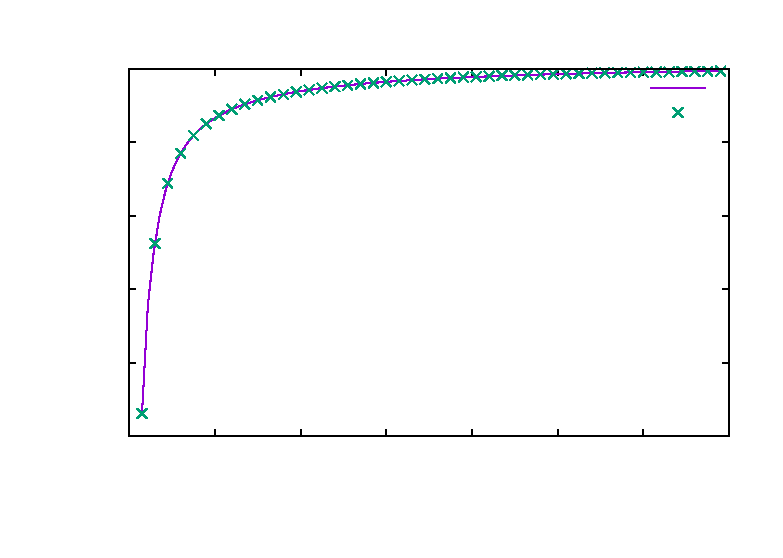
\includegraphics{plot-gnuplottex-fig1}}%
    \gplfronttext
  \end{picture}%
\endgroup
